\documentclass[a4paper,12pt]{article} % тип документа

% Поля страниц
\usepackage[left=2.5cm,right=2.5cm, top=2cm,bottom=2cm,bindingoffset=0cm]{geometry}

%Пакет дял таблиц   
\usepackage{multirow} 

%Отступ после заголовка    
\usepackage{indentfirst}


% Рисунки
\usepackage{subcaption,floatrow,graphicx,calc}
\usepackage{wrapfig}

% Создаёем новый разделитель
\DeclareFloatSeparators{mysep}{\hspace{1cm}}

% Ссылки?
\usepackage{hyperref}
\usepackage[rgb]{xcolor}
\hypersetup{				% Гиперссылки
	colorlinks=true,       	% false: ссылки в рамках
	urlcolor=blue          % на URL
}


%  Русский язык
\usepackage[T2A]{fontenc}			% кодировка
\usepackage[utf8]{inputenc}			% кодировка исходного текста
\usepackage[english,russian]{babel}	% локализация и переносы


% Математика
\usepackage{amsmath,amsfonts,amssymb,amsthm,mathtools, mathrsfs, wasysym}


\begin{document}
	\begin{center}
		\footnotesize{ФЕДЕРАЛЬНОЕ ГОСУДАРСТВЕННОЕ АВТОНОМНОЕ ОБРАЗОВАТЕЛЬНОЕ 			УЧРЕЖДЕНИЕ ВЫСШЕГО ОБРАЗОВАНИЯ}\\
		\footnotesize{МОСКОВСКИЙ ФИЗИКО-ТЕХНИЧЕСКИЙ ИНСТИТУТ\\(НАЦИОНАЛЬНЫЙ 			ИССЛЕДОВАТЕЛЬСКИЙ УНИВЕРСИТЕТ)}\\
		\footnotesize{ФАКУЛЬТЕТ ОБЩЕЙ И ПРИКЛАДНОЙ ФИЗИКИ\\}
		\hfill \break
		\hfill\break
		\hfill\break
		\hfill \break
		\hfill \break
		\hfill \break
		\hfill \break
		\hfill \break
		\hfill \break
		\hfill \break
		\hfill \break
		\hfill \break
		\hfill \break
		\hfill \break
		\large{Лабораторная работа № 6.11.1 \\\textbf{Определение ширины запрещенной зоны полупроводника}}\\
		\hfill \break
		\hfill \break
		\hfill \break
		\begin{flushright}
			Серебренников Даниил\\
			Группа Б02-826м
		\end{flushright}
		\hfill \break
		\hfill \break
		\hfill \break
		\hfill \break
		\hfill \break
		\hfill \break
		\hfill \break
		\hfill \break
		\hfill \break
		\hfill \break
		\hfill \break
	\end{center}
	\begin{center}
		Долгопрудный, 2021 г.
	\end{center}
	\thispagestyle{empty}
	\newpage
	\textbf{Цель работы:} исследовать температурную зависимость проводимости типичного полупроводника -- германия или кремния. Определить ширину запрещенной зоны с помощью цифрового вольтметра.
	
	\section{Основные формулы}
	Удельная проводимость образца:
	\begin{equation*}
		\sigma = \frac{l}{RS},
	\end{equation*}
	где $R$ -- сопротивление образца, $l$ -- его длина, а $S$ -- поперечное сечение.
	
	Ширина запрещающей зоны:
	\begin{equation*}
		\label{delta}
		\tag{$\star$}
		\Delta = 2k \frac{\Delta(\ln \sigma)}{\Delta (1/T)}.
	\end{equation*}
	\section{Экспериментальная установка}
	\thisfloatsetup{floatrowsep=mysep}	
	\begin{figure}[h!]
		\begin{floatrow}
			\ffigbox[\FBwidth]{\caption{Схема экспериментальной установки.}\label{fig:ust}}
			{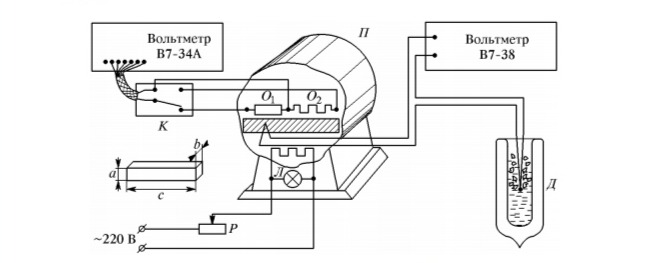
\includegraphics[scale=0.7]{ustanovka}}    
		\end{floatrow}
	\end{figure}
	
	
	\newpage
	\section{Экспериментальные данные}
	\begin{enumerate}
		\item
		$\sigma_{R} = 0,001$ кОм;
		\item
		$\sigma_V = 0,01$ мВ;
		\item
		Коэффициент термопары
		$\lambda = 41$ мкВ/$^\circ$C;
		\item
		Температура термометра $t_0 = (26,0 \pm 0,5)^\circ$C.
		\item
		Параметры образца $l = 39,2$ мм, $S = 4,1\cdot4,1$ мм$^2$.
	\end{enumerate}
	
	\floatsetup[table]{capposition=top}	
	\begin{table}[H]
		\caption{Результаты измерений.}
		\label{table:exp1}
		\begin{tabular}{|c|c|c|c|c|c|c|}
			\hline
			$R$, кОм & $V$, мВ & $t$, $^\circ$C & $T$, К & $\sigma$, $(\text{Ом}\cdot\text{м})^{-1}$ & $1/T$, К$^{-1}$ & $\ln \sigma$ \\ \hline
			0,769    & -0,10   & 23,6           & 296,6  & 3,03                                      & 0,003372        & 1,11         \\ \hline
			0,639    & 0,05    & 27,2           & 300,2  & 3,65                                      & 0,003331        & 1,29         \\ \hline
			0,565    & 0,02    & 26,4           & 299,4  & 4,13                                      & 0,003340        & 1,42         \\ \hline
			0,469    & 0,30    & 33,3           & 306,3  & 4,97                                      & 0,003265        & 1,60         \\ \hline
			0,339    & 0,58    & 40,1           & 313,1  & 6,88                                      & 0,003193        & 1,93         \\ \hline
			0,318    & 0,64    & 41,6           & 314,6  & 7,33                                      & 0,003179        & 1,99         \\ \hline
			0,296    & 0,70    & 43,1           & 316,1  & 7,88                                      & 0,003164        & 2,06         \\ \hline
			0,189    & 1,15    & 54,0           & 327,0  & 12,34                                     & 0,003058        & 2,51         \\ \hline
			0,149    & 1,40    & 60,1           & 333,1  & 15,65                                     & 0,003002        & 2,75         \\ \hline
			0,099    & 1,85    & 71,1           & 344,1  & 23,56                                     & 0,002906        & 3,16         \\ \hline
			0,075    & 2,20    & 79,7           & 352,7  & 31,09                                     & 0,002836        & 3,44         \\ \hline
			0,055    & 2,61    & 89,7           & 362,7  & 42,40                                     & 0,002757        & 3,75         \\ \hline
			0,042    & 3,00    & 99,2           & 372,2  & 55,52                                     & 0,002687        & 4,02         \\ \hline
			0,032    & 3,40    & 108,9          & 381,9  & 72,87                                     & 0,002618        & 4,29         \\ \hline
			0,025    & 3,80    & 118,7          & 391,7  & 93,28                                     & 0,002553        & 4,54         \\ \hline
			0,023    & 4,00    & 123,6          & 396,6  & 101,39                                    & 0,002522        & 4,62         \\ \hline
			0,021    & 4,20    & 128,4          & 401,4  & 111,05                                    & 0,002491        & 4,71         \\ \hline
			0,018    & 4,40    & 133,3          & 406,3  & 129,55                                    & 0,002461        & 4,86         \\ \hline
			0,017    & 4,60    & 138,2          & 411,2  & 137,17                                    & 0,002432        & 4,92         \\ \hline
			0,015    & 4,80    & 143,1          & 416,1  & 155,46                                    & 0,002403        & 5,05         \\ \hline
			0,014    & 5,00    & 148,0          & 421,0  & 166,57                                    & 0,002376        & 5,12         \\ \hline
		\end{tabular}
	\end{table}
	
	
	
	\newpage
	\section{Обработка результатов}
		\thisfloatsetup{floatrowsep=mysep}	
		\begin{figure}[h!]
			\begin{floatrow}
				\ffigbox[\FBwidth]{\caption{Зависимость $\sigma$ от $T$.}\label{fig:f(x)1}}
				{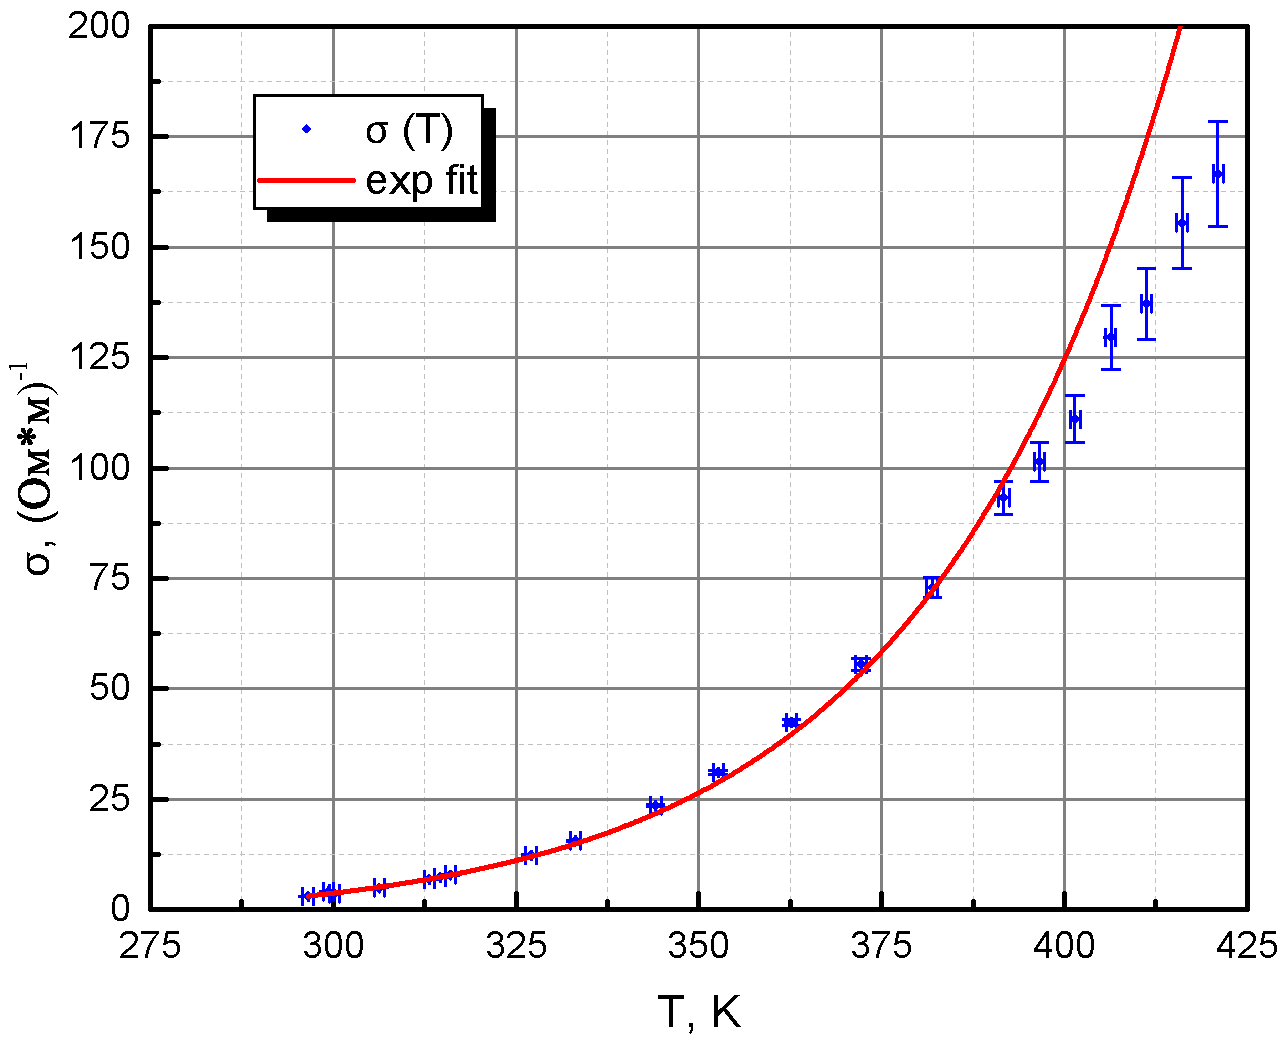
\includegraphics[scale=0.5]{graph1.pdf}}    
			\end{floatrow}
		\end{figure}
	
		\thisfloatsetup{floatrowsep=mysep}	
		\begin{figure}[h!]
			\begin{floatrow}
				\ffigbox[\FBwidth]{\caption{Зависимость $\ln \sigma$ от $1/T$.}\label{fig:f(x)2}}
				{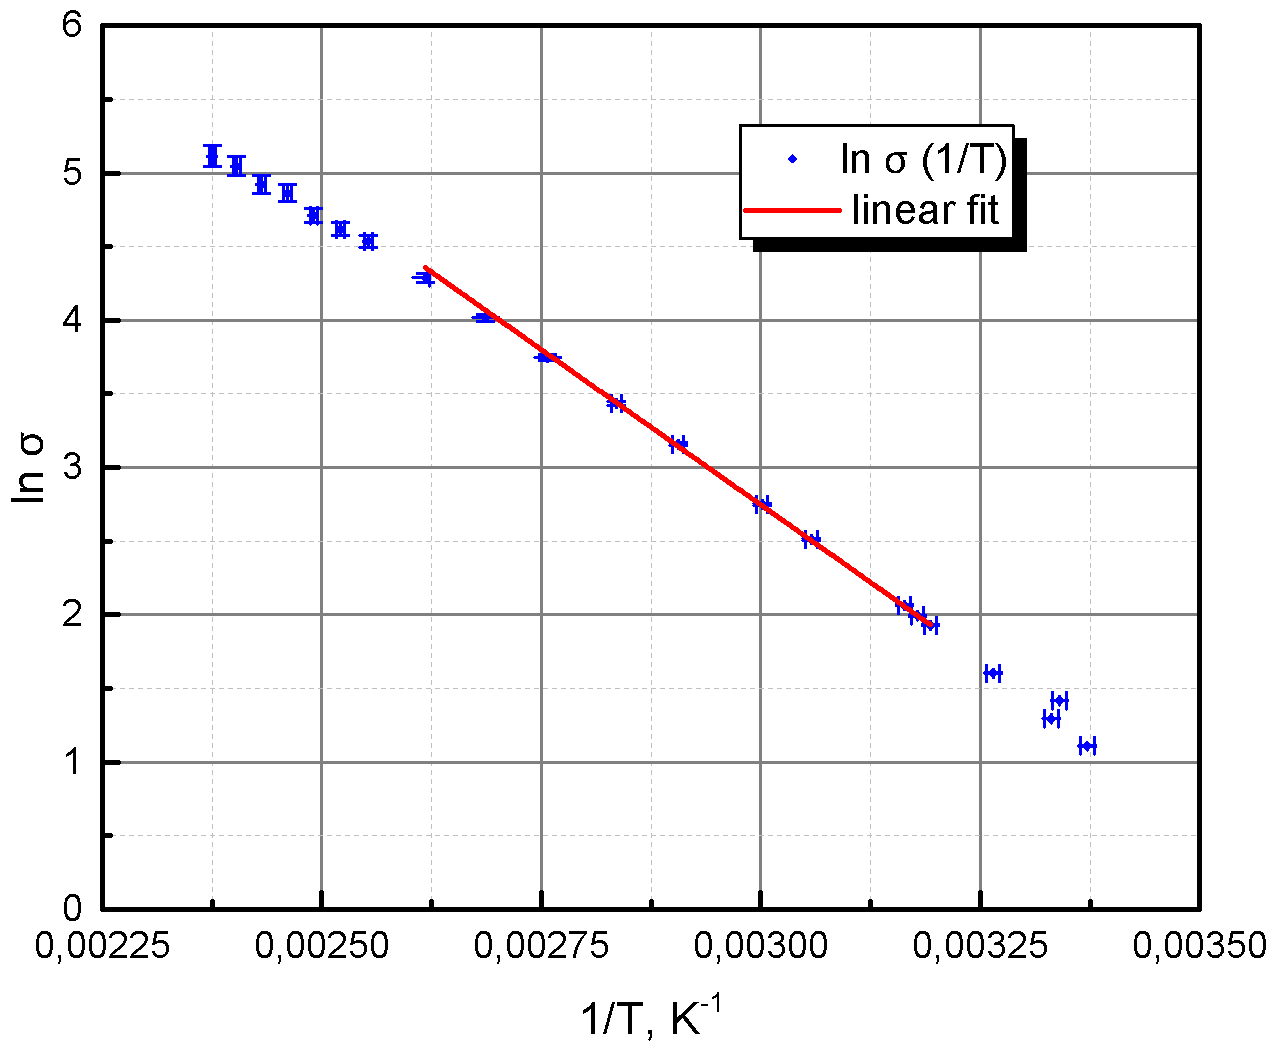
\includegraphics[scale=0.5]{graph2.pdf}}    
			\end{floatrow}
		\end{figure}
		Наклон прямой есть $(-4220 \pm 30)$ К, тогда ширина запрещенной зоны, согласно формуле ~(\ref{delta}) есть \[\boxed{\Delta = (0,724 \pm 0,006)\text{эВ}}\].
	
	
	
	
	
	
	
	
	\newpage
	\section{Обсуждение результатов и выводы}
		Исследована температурная зависимость проводимости типичного полупроводника - германия или крмения. Определена ширина запрещающей зоны, которая несколько завышает табличное значение.
		
		Стоит отметить, что на рисунке ~\ref{fig:f(x)1} наблюдается переход экспоненты в прямую. Это обусловлено тем, что при выскоих температурах происходит вырождение полупроводника в полуметалл.
	
\end{document}